\chapter{Prestudy}

\label{prestudy}

A thorough study of the problem area, existing solutions, development methods etc. is important to gain the knowledge needed to make good decisions concerning the project. In this chapter the research preformed in the first phase of the project will be presented.

\section{Development methods}
Several development methods were examined in the beginning of the project to ensure that a suitable model was chosen. In the following section the research performed on different development methods will be presented. Regarding the choice of development method, the decision of the group will be presented in Chapter \ref{development-method}.

\subsection{Rational Unified Process}
Rational Unified Process (RUP) is an iterative and incremental software development process model. It is a process model that aims to capture the best practises in modern software development and present them in a tailorable form.\cite{kruchten} Each iteration in this model results in an increment, which is a release of a prototype and an improvement of the previous iteration. Most of the iterations will, in addition to work on prototypes, also contain work on requirements, design, implementation, testing and so on.\\
\newline
A feature of this model is that it is use case driven. Every iteration takes a set of use case scenarios from the requirements and use those for the content of the iteration. The model also requires the team to focus on the critical risks of the project early in the development process. This ensures that problem areas and uncertainties is dealt with before severe problems arise. An illustration of the model is shown in Figure~\ref{fig:rup}.
\newline
The model consists of four phases:

\begin{itemize}
\item{Inception}
\item{Elaboration}
\item{Construction}
\item{Transition}
\end{itemize}

\paragraph{Inception phase} The inception phase is the smallest phase, and should cover the work on identifying risks, creating use cases, establish boundaries and so on. Cost estimates is calculated in the inception phase. This phase should result in a document that states the core of the product, with an preliminary overview of the architecture, requirements, use cases and risks.

\paragraph{Elaboration phase} In the Elaboration phase the team is expected to filter out the majority of the system requirements and validate the system architecture. A detailed overview of the product should be established in this phase, and the project plan should be developed. The documentation produced in this phase is essential for the work done in the Construction phase.

\paragraph{Construction phase} The Construction phase is the largest phase in the model. In this phase all the remaining features of the product are developed and integrated, and thoroughly tested. At the end of this phase, the finished product should be ready to be presented to the customer.

\paragraph{Transition phase} The Transition phase is where the system is deployed to the target users. Feedback from the customer might result in further refinements, and new versions of the product. Elements in this phase is beta testing and training of the users.

\begin{figure}[H]
\centering
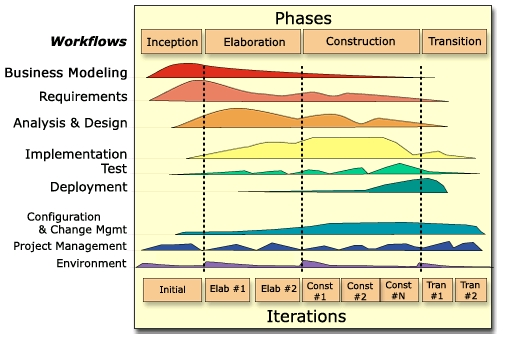
\includegraphics[scale=0.7]{images/rup.jpg}
\caption{Rational Unified Process}
\label{fig:rup}
\end{figure}

\subsection{Scrum}
Scrum is an iterative and incremental development framework for development of complex information systems. When using Scrum, the development of the product is developed in small pieces, with each piece building upon previously created pieces. The use of Scrum requires the team to be divided into specific roles, where each role has its own responsibility. The following are the core roles of the Scrum team\cite{scrum}\cite{sommerville}:
\begin{description}
	\item[Product owner:]{The product owner represents the stakeholders in the project, and is the voice of the customer. It is the product owner's responsibility to ensure that the Scrum team at all times is working with the right things seen from a business perspective.}
	\item[Scrum master:]{The scrum master should act as a buffer between the development team and distracting influences, so that the development team can deliver potentially shippable products at the end of each sprint. The scrum master should keep the development team focused at all times.}
	\item[Development team:]{The development team is made up from three to nine persons with cross-functional skills. This team does all the actual work, including development, testing, designing and so on.}
\end{description}

\subsection{Waterfall model}
The waterfall model is among the first process models to be introduced. In this model, each phase in the development must be completed before one can advance to the next phase. At the end of each phase in the development, a review takes place. In this review it is determined if the project is on the right path and if it should continue or not. The phases in the development do not overlap. \cite{sommerville}

\subsection{Spiral model}
The spiral model is a software development model intended for large and complicated projects. It combines elements from the waterfall model and prototyping models, and uses an iterative approach. Based on this it allows for incremental releases of the product, as prototypes. \cite{sommerville}

%Check if it is written anything about this in the Systemutviklings-bok.
\subsection{Lean software development}
\label{leandev}
Lean is an agile software development methodology that is defined by seven principles\cite{poppendieck}:
\begin{description}
	\item[Eliminate waste.]{Everything that does not add any value to the customer is considered a waste.}
	\item[Amplify learning.]{The development environment should the designed so it amplifies the learning process of the developers. Defects should be prevented by running tests as soon as the code is written.}
	\item[Decide as late as possible.]{By delaying decisions as much as possible, better results can be achieved. There is always uncertainty associated with software development, and delaying options as much as possible results in more flexibility later.}
	\item[Deliver as fast as possible.]{The sooner the product is delivered, the sooner feedback can be received.}
	\item[Empower the team.]{The managers are taught how to listen to the developers, so they can explain better what actions could be taken and give suggestions for improvements.}
	\item[Build integrity.]{The customer needs to have influence and inspection of the project, and an overall experience of the system to be developed.}
	\item[See the whole.]{Decompose the system into smaller parts and find and eliminate defects.}
\end{description}

\section{Existing solutions}
This is a summary of existing solutions similar to the project assignment. This section is divided in two subsections; one for the market application and one for the over-the-air transfer. The existing products were evaluated on the following criteria:
\begin{itemize}
	\item{To what degree the product fits the assignment.}
	\item{Can the product, or parts of it, be reused for the assignment? Can it lead to licensing issues?}
\end{itemize}

\subsection{Market applications}
\paragraph{UbiBazaar} is a prior project which created an universal app store in PHP. This project had potential for serving as a back end, but this was later discarded. The idea of a website for uploading applications was the primary idea for the project. Upon revising the project it was deemed too unstable and incomplete to properly function for our intended use. The project used an outdated version of PHP which caused numerous bugs which would take up too much time to attempt to fix properly.\\

It did have a way for developers to follow each other, which would help creating a community for the developers. For further development of $\mu$CSS, UbiBazaar would also be able to support the development of applications aimed at, for example, raspberry pi. This was not included as the goal of our project and therefore discarded.

\paragraph{Google Play} is the market application for Android provided by Google. It is an application that allows for easy browsing and installation of applications on Android devices. It also detects what model of phone that is being used, and only shows applications that are supported by that phone. This functionality is similar to the requirements for the Android application in the project.

\begin{figure}[H]
\centering
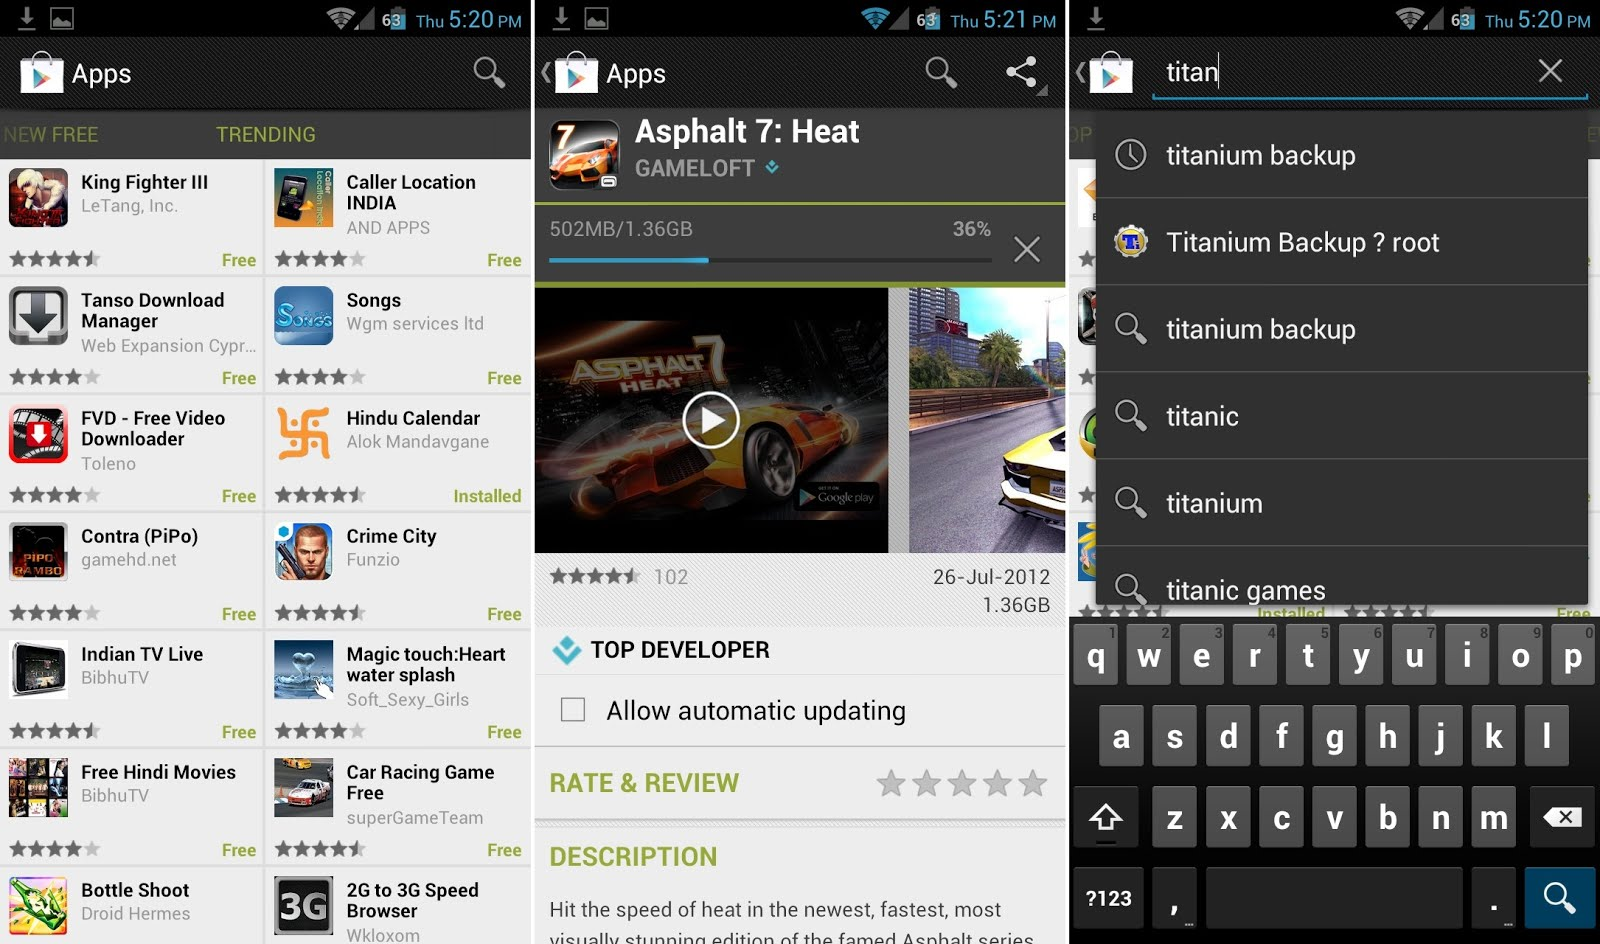
\includegraphics[scale=0.2]{images/Google-Play-Store-APK-3-7-15.jpg}
\caption{Google Play Store}
\label{fig:googleplay}
\end{figure}

Google Play fits the assignment in the way that is is a market applications where one can download applications. This was useful for the development of the product, since it was possible to use the same principles in the assignment. It was also similar in the way that it was possible to browse for applications on the computer, and ``push'' the application to a mobile telephone. This, however, did not connect via Bluetooth$\textsuperscript{\textregistered}$, as the task assignment stated the finished product should. Google Play is not open source and could therefore only be used as a source of inspiration for the project. It was not possible to reuse the code or other parts of the application in the development.


\subsection{Pebble}
Pebble is a watch that offers over the air transfer of applications. The main differences between this watch and a standard Arduino$\texttrademark$, is that Pebble have written a custom operating system in C for this device and contains a Bluetooth$\textsuperscript{\textregistered}$ connection. Pebble is also using a microcontroller that is significantly faster and contains a lot more memory, which means that it is much easier to develop an operating system for it.\\
\\
To transfer a new application to the watch, the user connects the mobile phone to the watch using Bluetooth$\textsuperscript{\textregistered}$. The user can then open the Pebble application store and upload applications made for this watch.

\begin{figure}[H]
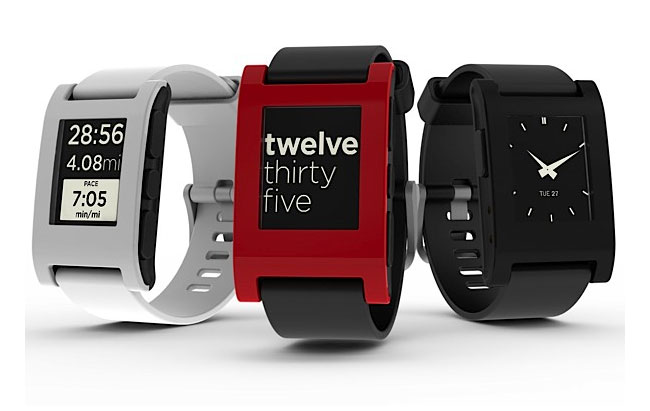
\includegraphics[scale=0.7]{images/Pebble-Smartphone-Watch.jpeg}
\caption{Pebble Watch}
\label{fig:pebblewatch}
\end{figure}
The principles are quite similar to what we planned to develop, but this platform is not made to expand to other platforms. There was very little documentation on the Pebble website, so the potential for reuse in this project appears minimal.

\section{Over the air transfer}
Usually when you program the Arduino$\texttrademark$ you use a computer with a USB-cable connected to the Arduino$\texttrademark$ board. This is used because it is a stable connection and a standardized cable that everybody has available. This project's main goal was to remove the cable when you are programming the Arduino$\texttrademark$ and move the software over to an Android device. To remove the USB-cable we had to use Bluetooth$\textsuperscript{\textregistered}$ to communicate between the devices.
\\
\begin{figure}[H]
\centering
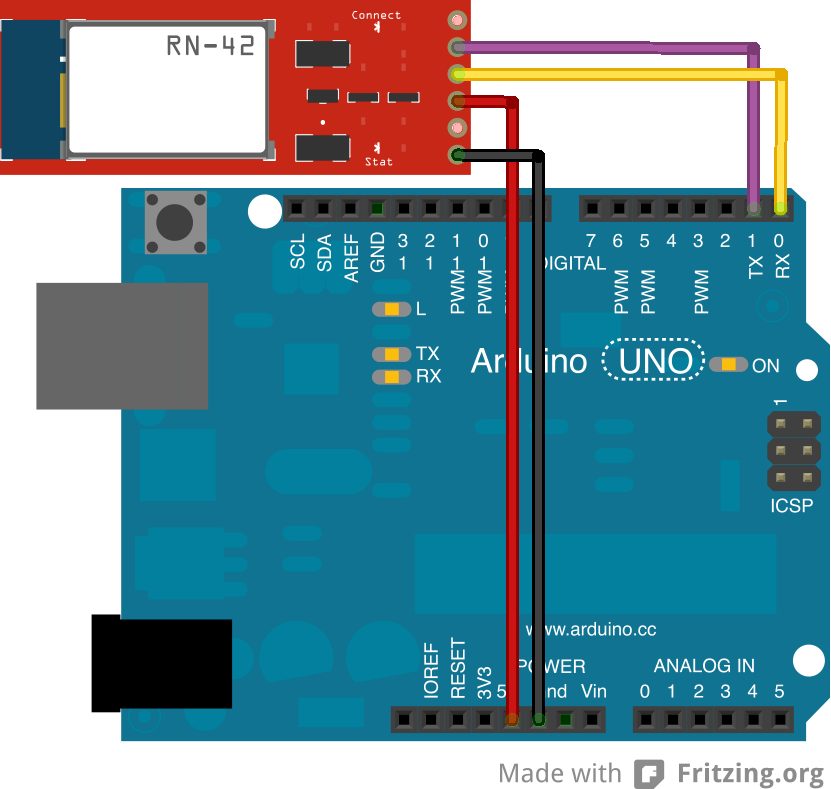
\includegraphics[scale=1.2]{images/wiring_simple.png}
\caption{Bluetooth$\textsuperscript{\textregistered}$ on Arduino$\texttrademark$}
\label{fig:SimpleArduinoWiring}
\end{figure}

% ref til RN-42
After a lot of research we made a wireless connection between the Android and the Arduino$\texttrademark$ with a Bluetooth$\textsuperscript{\textregistered}$ module, with the wiring as shown in figure~\ref{fig:SimpleArduinoWiring}. We used the Bluetooth$\textsuperscript{\textregistered}$ module RN-42 because it was well documented and easy to connect to the Arduino$\texttrademark$.\\
\\
The protocol to upload new code to the microcontroller is quite advanced. This must be done without any errors and with the correct baud rate, therefore we rely on the stability of the wireless communication. If an error occurs while uploading the code, it has to start over again.
